\documentclass[12pt]{jarticle}
\usepackage{TUSIreport}
\usepackage{otf}
\usepackage[dvipdfmx]{graphicx}
\usepackage[dvipdfmx]{color}
\usepackage{amsmath}
\usepackage{amssymb}
\usepackage{color}
\usepackage{hhline}
\usepackage{fancybox,ascmac}
\usepackage{multirow}
\usepackage{url}
\usepackage{bm}
\usepackage{listings,jlisting}
%%%%%%%%%%%%%%%%%%
\lstdefinestyle{py}{
    language={Python},
    backgroundcolor={\color[gray]{.85}},
    basicstyle={\small},
    identifierstyle={\small},
    commentstyle={\small\ttfamily \color[rgb]{0,0.5,0}},
    keywordstyle={\small\bfseries \color[rgb]{1,0,0}},
    ndkeywordstyle={\small},
    stringstyle={\small\ttfamily \color[rgb]{0,0,1}},
    frame={tb},
    breaklines=true,
    columns=[l]{fullflexible},
    numbers=left,
    xrightmargin=0zw,
    xleftmargin=3zw,
    numberstyle={\scriptsize},
    stepnumber=1,
    numbersep=1zw,
    morecomment=[l]{//}
}
\begin{document}
%%%%%%%%%%%%%%%%%%%%%%%%%%%%%%%%%%%%%%%%%%%%%%%%%%%%%%%%
% 表紙を出力する場合は,\提出者と\共同実験者をいれる
% \提出者{科目名}{課題名}{提出年}{提出月}{提出日}{学籍番号}{氏名}
% \共同実験者{一人目}{二人目}{..}{..}{..}{..}{..}{八人目}
%%%%%%%%%%%%%%%%%%%%%%%%%%%%%%%%%%%%%%%%%%%%%%%%%%%%%%%
\提出者{情報工学実験3}{課題4 画像変換}
{2021}{5}{6}{4619055}{辰川力駆}
%%%%%%%%%%%%%%%%%%%%%%%%%%%%%%%%%%%%%%%%%%%%%%%%%%%%%%%%%
\共同実験者{}{}{}{}{}{}{}{}
%%%%%%%%%%%%%%%%%%%%%%%%%%%%%%%%%%%%%%%%%%%%%%%%%%%%%%%%%
% 表紙を出力する場合はコメントアウトしない
%%%%%%%%%%%%%%%%%%%%%%%%%%%%%%%%%%%%%%%%%%%%%%%%%%%%%%%%%
\表紙出力
%%%%%%%%%%%%%%%%%%%%%%%%%%%%%%%%%%%%%%%%%%%%%%%%%%%%%%%
% 以下はレポート本体,reportmain.tex に書いてある.
% \inputを使っているが,直接書いても良い.
%%%%%%%%%%%%%%%%%%%%%%%%%%%%%%%%%%%%%%%%%%%%%%%%%%%%%%%
\section{実験の要旨}

入力画像やそのパラメータを変化させながら変換結果を比較し、
主観的な評価を行う。
それらを表にまとめ、考察をする。

\section{実験の目的}

画像変換の処理を題材に、
画像処理のプログラミングと評価を通じて、
画像処理の基本的な考え方を理解することを目的とする。

第3回目の実験では、
画像の2次元フーリエ変換と周波数フィルタリングを実装し、
入力画像やそのパラメータを変化させながら変換結果を評価することで、
フーリエ変換と周波数領域での画像処理について理解することを目的とする。

\section{課題1}
\subsection{実験方法}

\begin{enumerate}
    \item 自分で撮影した2枚の画像を合成してハイブリッド画像を作成する。
          \begin{enumerate}
              \item 自分で撮影した画像をPCにコピー(ダウンロード)する。
              \item ペイントソフト等を使って正方形の領域を切り出し、
                    必要に応じてグレースケール画像に変換し、
                    JPGファイル等に保存する。
              \item ハイブリッド画像を合成・表示する。
              \item ローパスフィルタ(LPF)、ハイパスフィルタ(HPF)のカットオフ周波数 cutoff1 、 cutoff2 を変化させると、
                    ハイブリッド画像の「認識しやすさ」がどのように変化するかを表にまとめる。
          \end{enumerate}
    \item 4組以上の画像について、ハイブリッド画像を作成し、
          どのような画像を用いると認識しやすいハイブリッド画像が合成できるか検討する。
\end{enumerate}

\begin{figure}[h]
    \begin{center}
        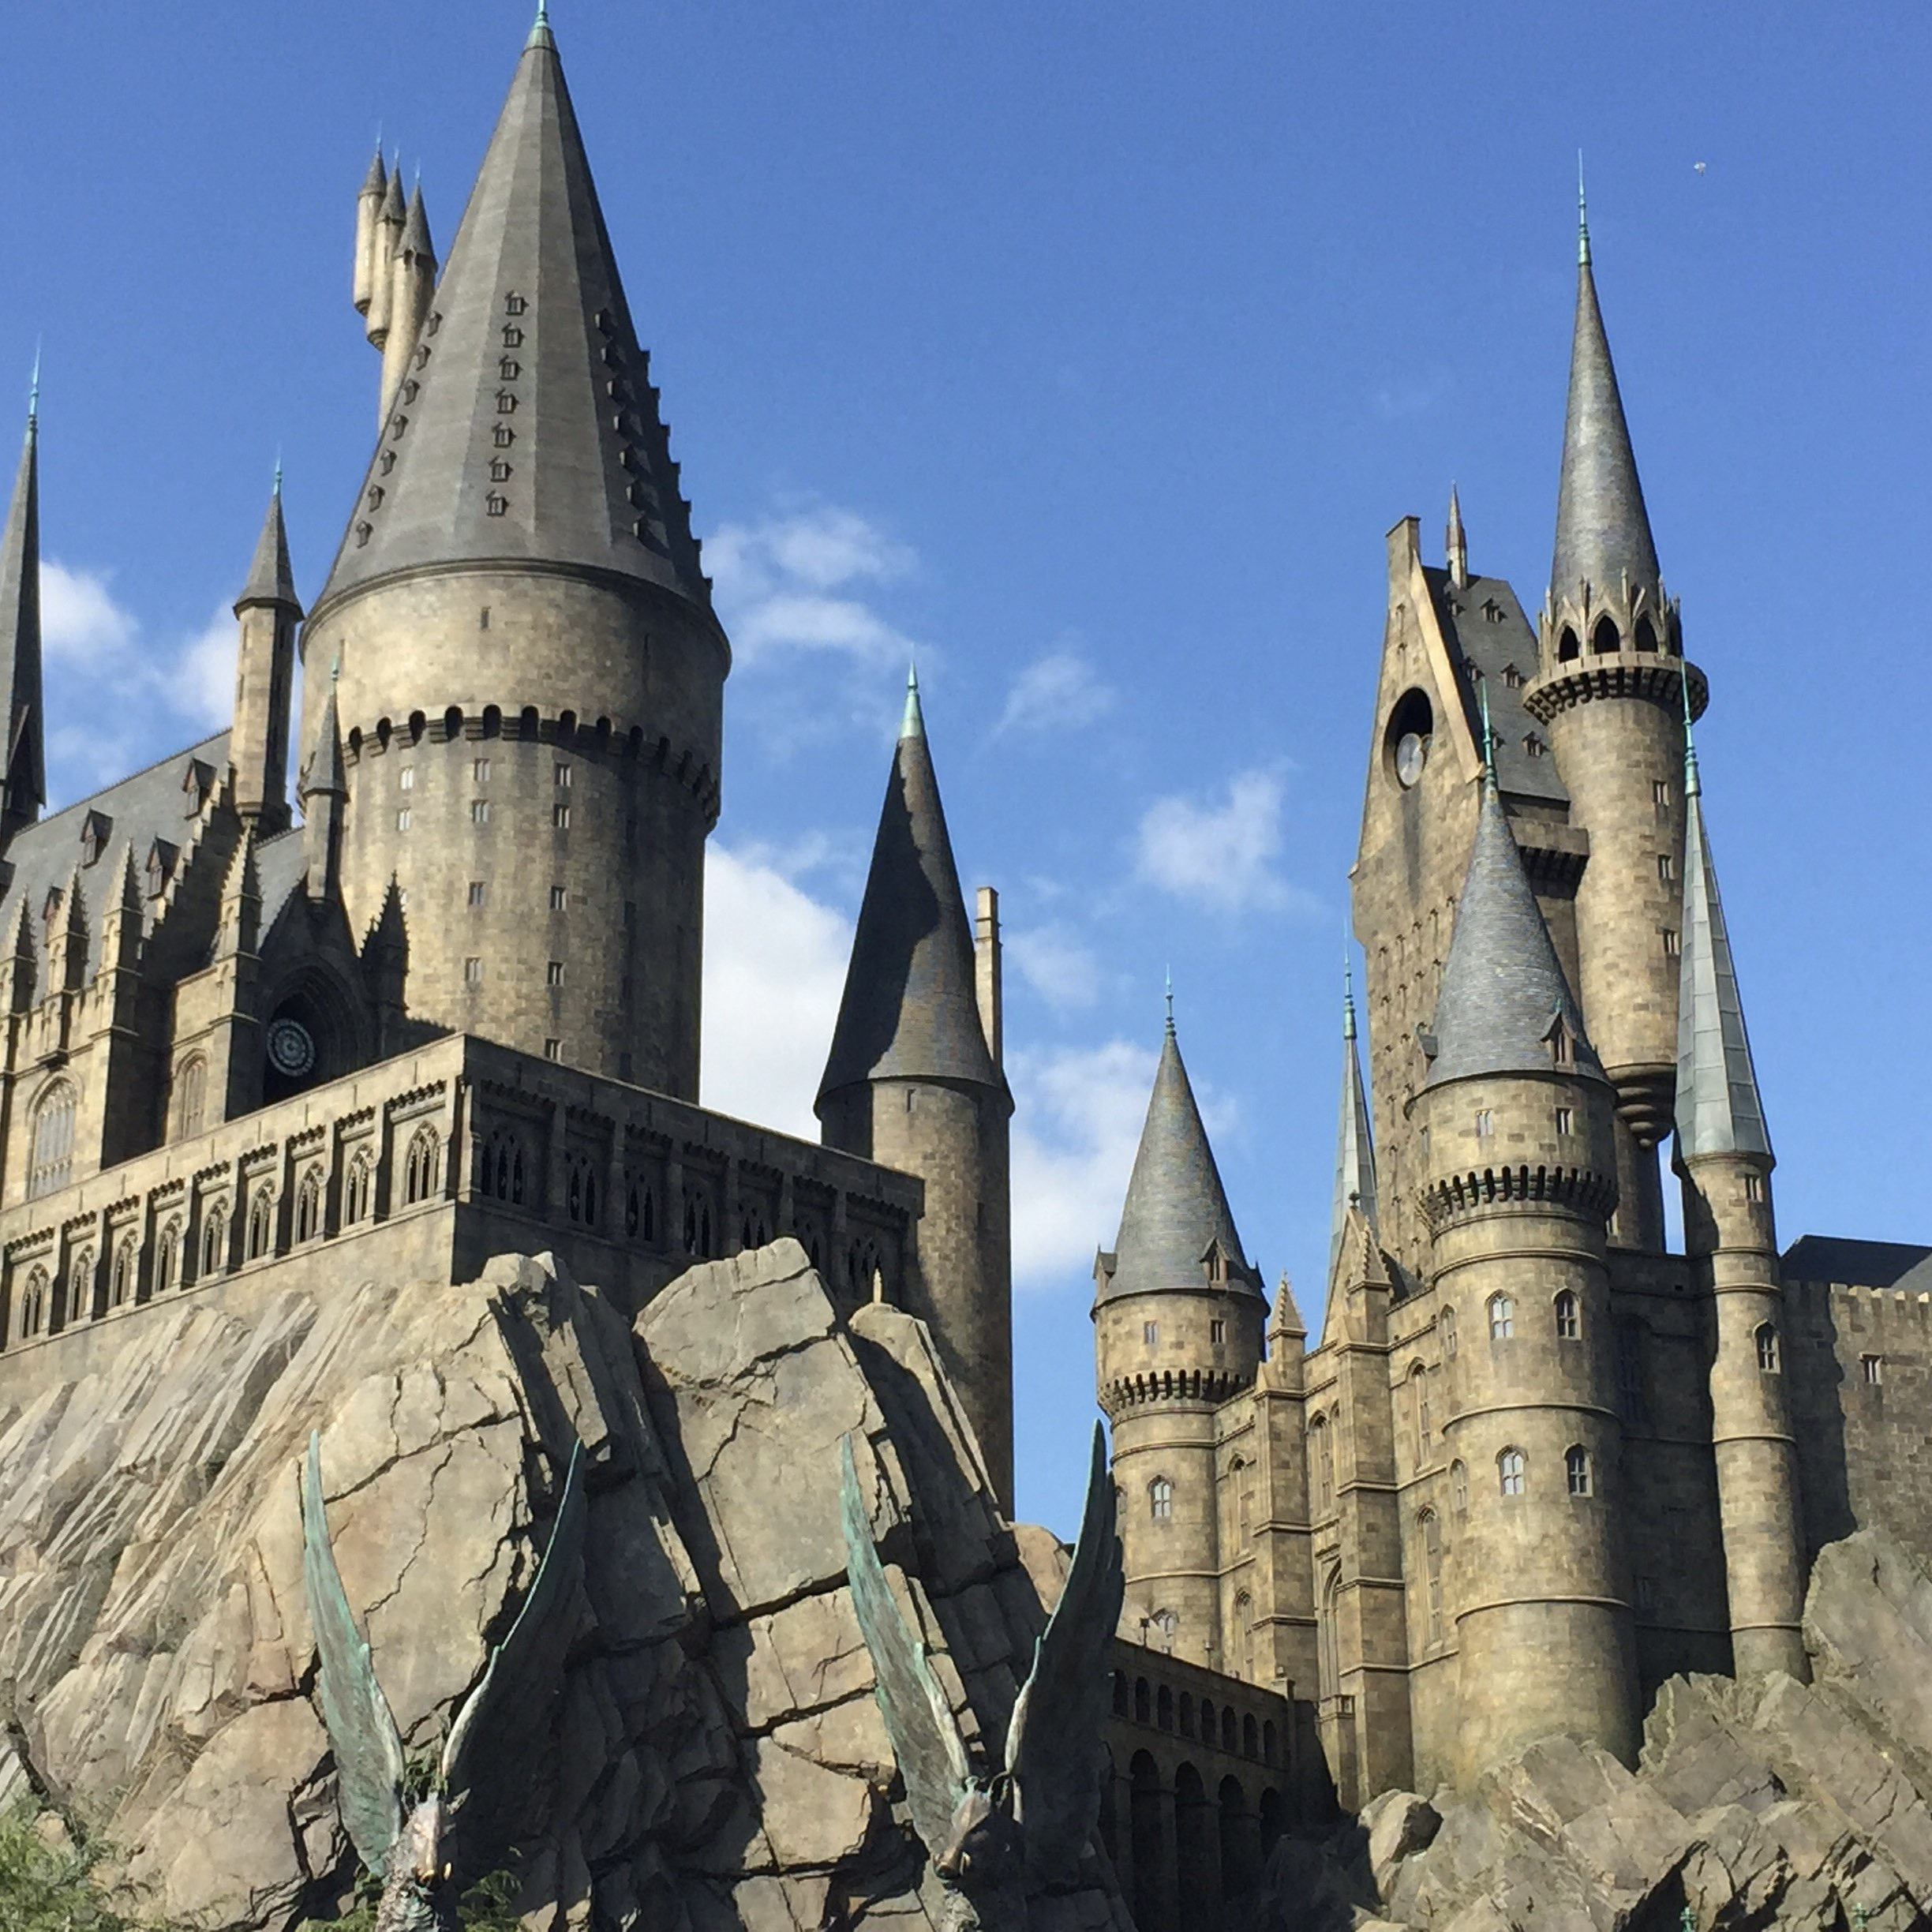
\includegraphics[scale=0.06]{kadai4_3_1.jpg}
    \end{center}
    \caption{画像1}
\end{figure}

\clearpage

\begin{figure}[h]
    \begin{center}
        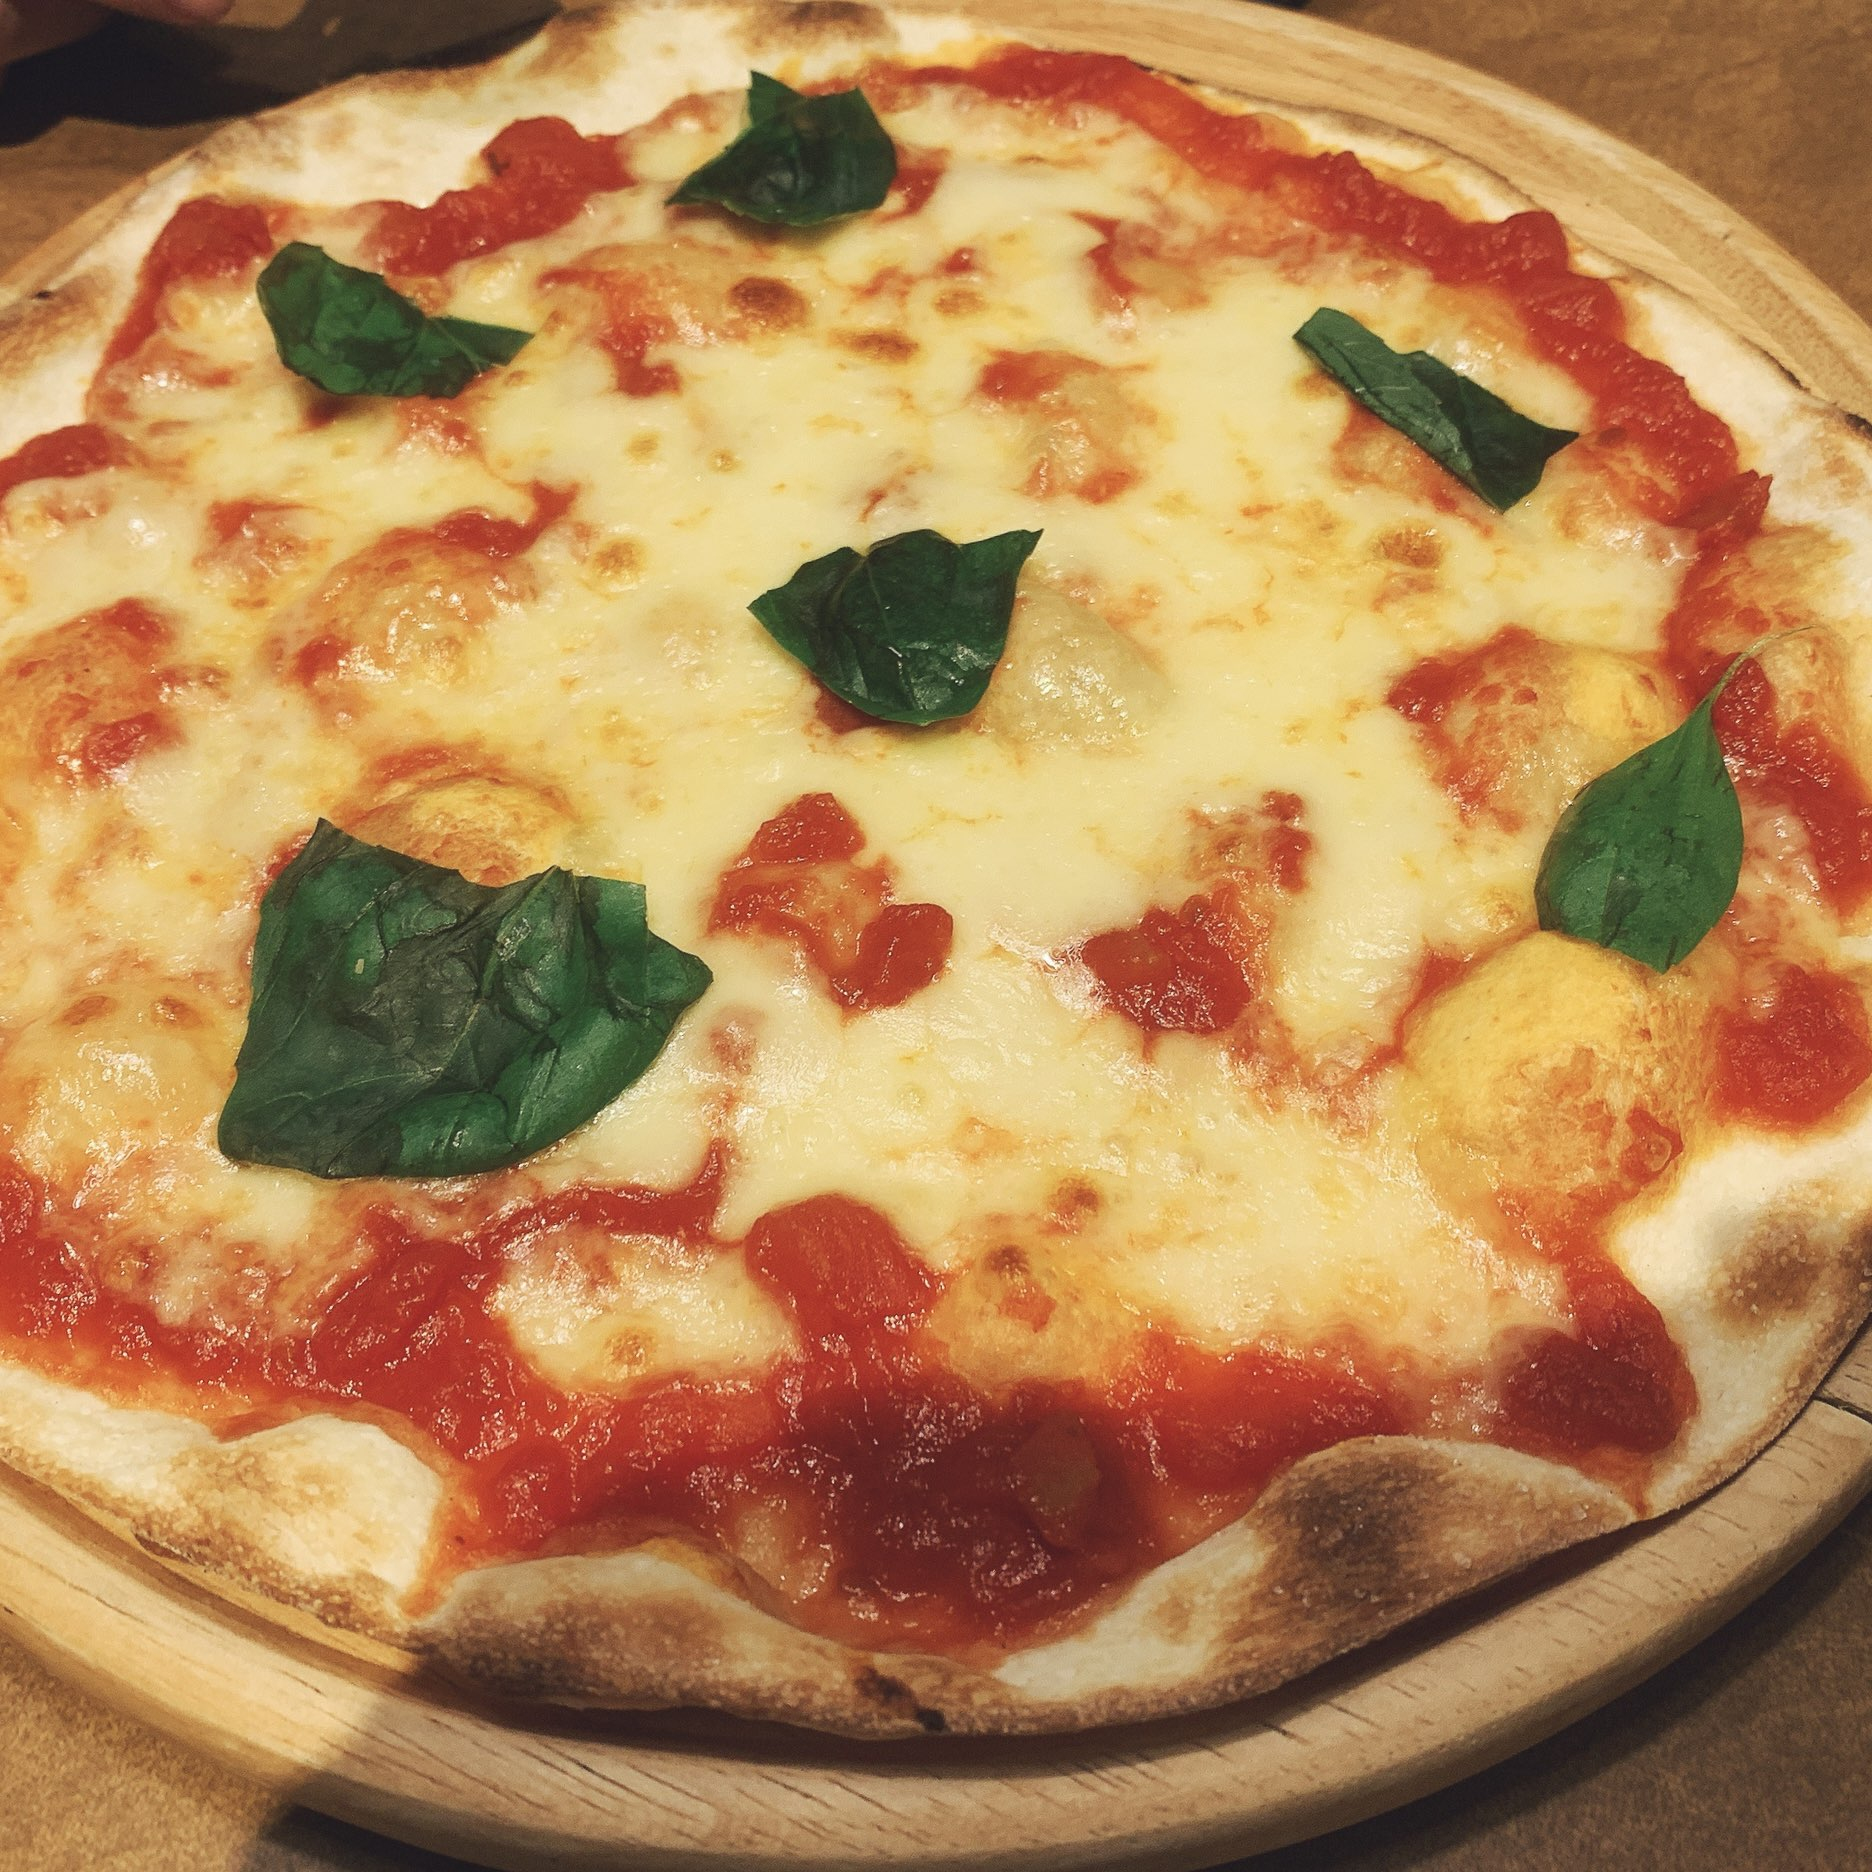
\includegraphics[scale=0.1]{kadai4_3_2.jpg}
    \end{center}
    \caption{画像2}
\end{figure}
\begin{figure}[h]
    \begin{center}
        
\includegraphics[scale=0.2]{kadai4_3_3.jpg}
    \end{center}
    \caption{画像3}
\end{figure}

\clearpage
\begin{figure}[h]
    \begin{center}
        
\includegraphics[scale=0.1]{kadai4_3_4.jpg}
    \end{center}
    \caption{画像4}
\end{figure}

\subsection{実験結果}

作成したプログラムは付録のソースコード1に載せた。

\subsubsection{}
用いる画像は、画像1と画像2である。
カットオフ周波数を変化させてハイブリッド画像を作成した。
実験条件として、モニター上の(一番左の)画像サイズは5.6[cm]、
被験者とモニターの間の距離は59.4[cm]である。
その実験下で、「認識しやすさ」と「カットオフ周波数」の関係について表1にまとめた。
これは、主観的なものであり、自分の意見である。
\begin{figure}[h]
    \begin{center}
        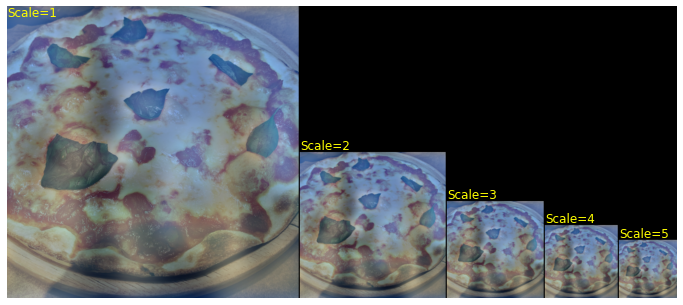
\includegraphics[scale=0.7]{kadai4_3_5.png}
    \end{center}
    \caption{cutoff1=4, cutoff2=8の結果}
\end{figure}

\begin{figure}[h]
    \begin{center}
        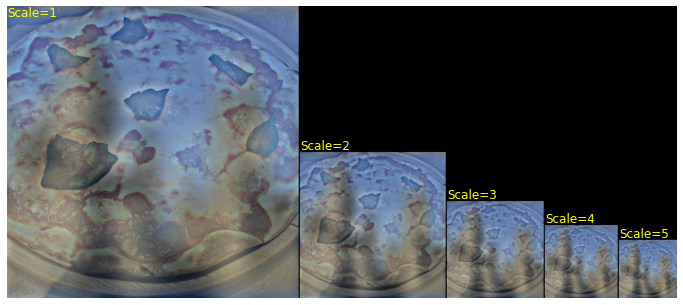
\includegraphics[scale=0.7]{kadai4_3_6.png}
    \end{center}
    \caption{cutoff1=4, cutoff2=16の結果}
\end{figure}

\clearpage
\begin{figure}[h]
    \begin{center}
        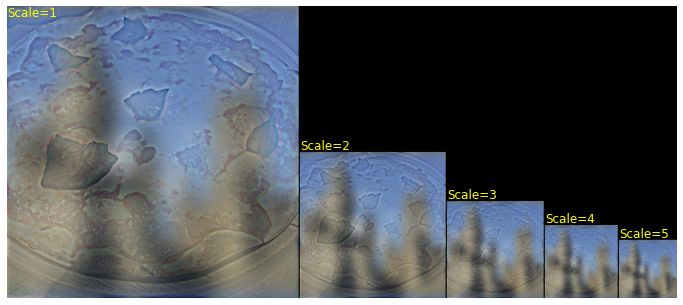
\includegraphics[scale=0.7]{kadai4_3_7.png}
    \end{center}
    \caption{cutoff1=4, cutoff2=32の結果}
\end{figure}

\begin{figure}[h]
    \begin{center}
        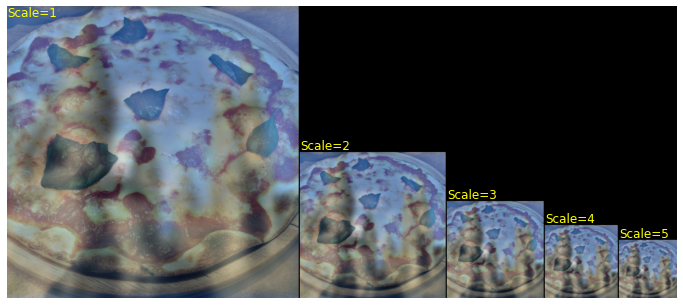
\includegraphics[scale=0.7]{kadai4_3_8.png}
    \end{center}
    \caption{cutoff1=8, cutoff2=8の結果}
\end{figure}

\clearpage
\begin{figure}[h]
    \begin{center}
        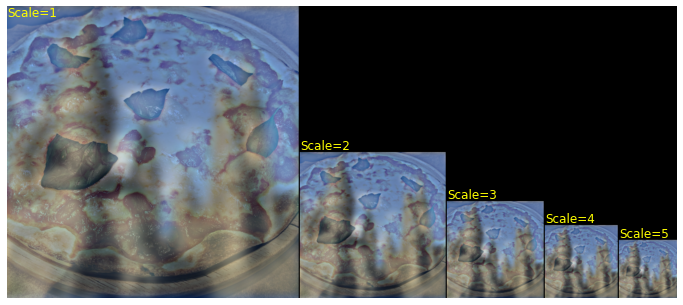
\includegraphics[scale=0.7]{kadai4_3_9.png}
    \end{center}
    \caption{cutoff1=8, cutoff2=16の結果}
\end{figure}

\begin{figure}[h]
    \begin{center}
        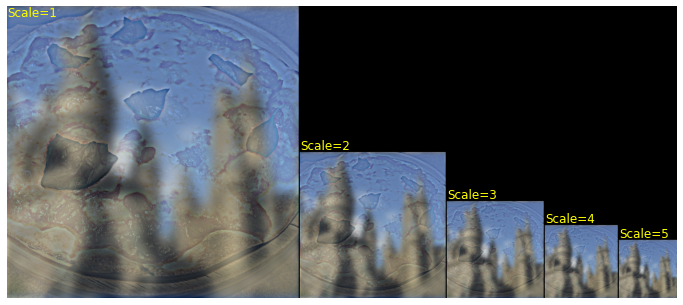
\includegraphics[scale=0.7]{kadai4_3_10.png}
    \end{center}
    \caption{cutoff1=8, cutoff2=32の結果}
\end{figure}

\clearpage
\begin{figure}[h]
    \begin{center}
        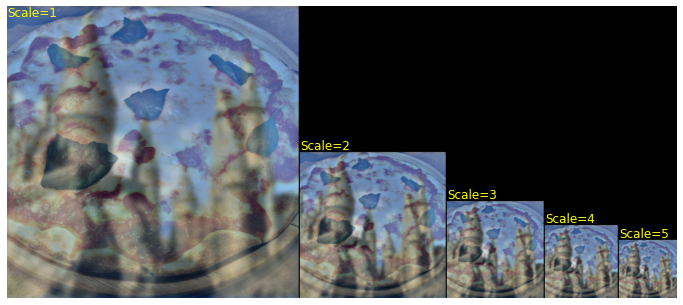
\includegraphics[scale=0.7]{kadai4_3_11.png}
    \end{center}
    \caption{cutoff1=16, cutoff2=8の結果}
\end{figure}

\begin{figure}[h]
    \begin{center}
        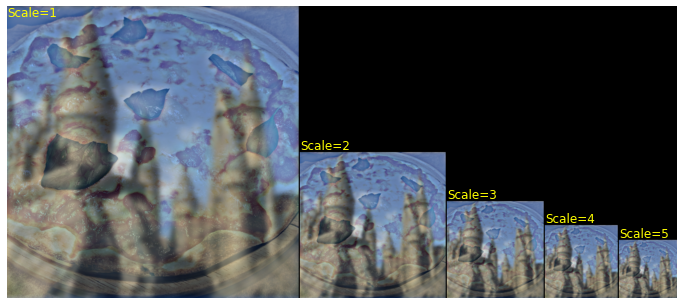
\includegraphics[scale=0.7]{kadai4_3_12.png}
    \end{center}
    \caption{cutoff1=16, cutoff2=16の結果}
\end{figure}

\clearpage
\begin{figure}[h]
    \begin{center}
        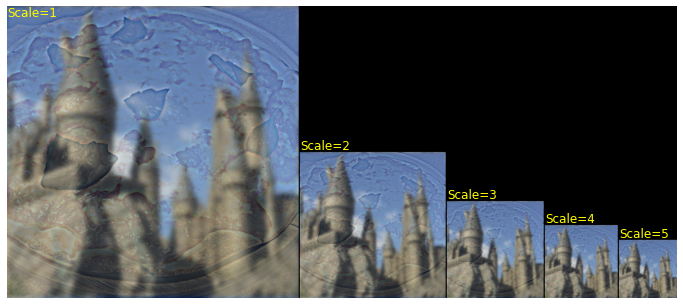
\includegraphics[scale=0.7]{kadai4_3_13.png}
    \end{center}
    \caption{cutoff1=16, cutoff2=32の結果}
\end{figure}

\begin{figure}[h]
    \begin{center}
        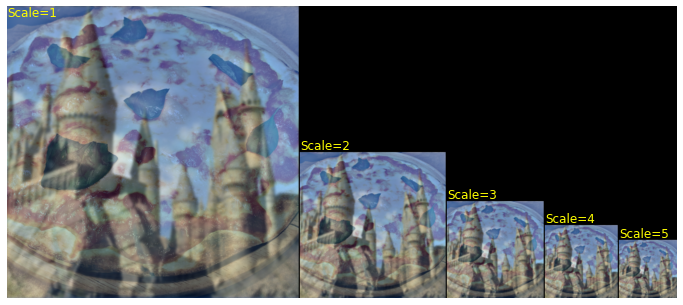
\includegraphics[scale=0.7]{kadai4_3_14.png}
    \end{center}
    \caption{cutoff1=32, cutoff2=8の結果}
\end{figure}

\clearpage
\begin{figure}[h]
    \begin{center}
        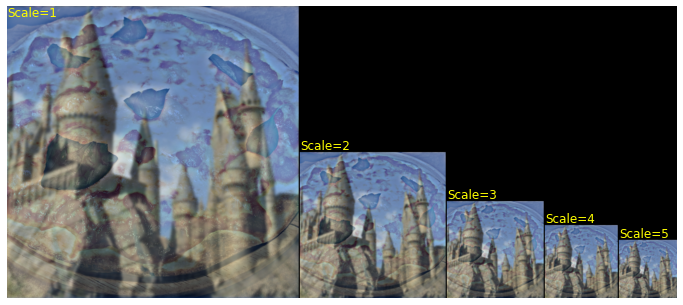
\includegraphics[scale=0.7]{kadai4_3_15.png}
    \end{center}
    \caption{cutoff1=32, cutoff2=16の結果}
\end{figure}

\begin{figure}[h]
    \begin{center}
        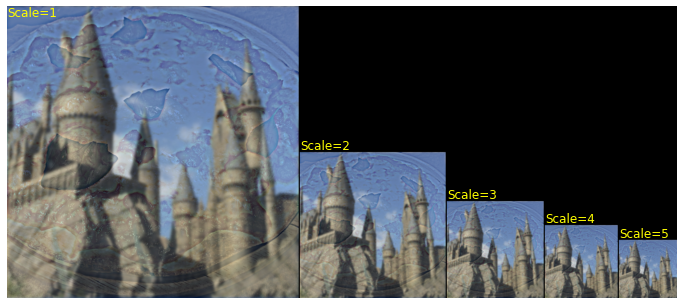
\includegraphics[scale=0.7]{kadai4_3_16.png}
    \end{center}
    \caption{cutoff1=32, cutoff2=32の結果}
\end{figure}

\clearpage
\begin{table}[htb]
    \caption{認識しやすさの評価結果}
    \begin{center}
        \begin{tabular}{|c||c|c|c|}
            \hline
            cutoff1 \textbackslash cutoff2 & 8  & 16 & 32 \\ \hline \hline
            4                              & 低 & 中 & 低 \\ \hline
            8                              & 中 & 中 & 低 \\ \hline
            16                             & 高 & 中 & 中 \\ \hline
            32                             & 中 & 中 & 低 \\ \hline
        \end{tabular}
    \end{center}
\end{table}

\subsubsection{}
カットオフ周波数はcutoff1=16、cutoff2=8として、4組の画像でハイブリッド画像を作成した。

\begin{itemize}
    \item [(1)]画像3と画像4を用いてハイブリッド画像を作成した。
          \begin{figure}[h]
              \begin{center}
                  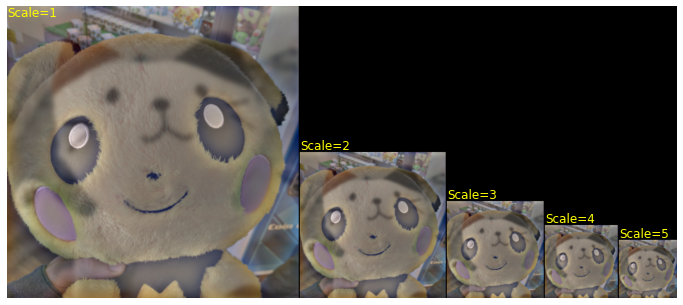
\includegraphics[scale=0.7]{kadai4_3_17.png}
              \end{center}
              \caption{(1)のハイブリッド画像}
          \end{figure}

          \clearpage
          \begin{figure}[h]
              \begin{center}
                  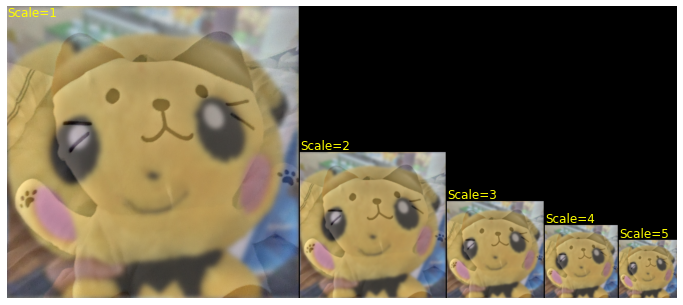
\includegraphics[scale=0.7]{kadai4_3_18.png}
              \end{center}
              \caption{(1)の入れ替えたハイブリッド画像}
          \end{figure}

    \item [(2)]画像2と画像3を用いてハイブリッド画像を作成した。
          \begin{figure}[h]
              \begin{center}
                  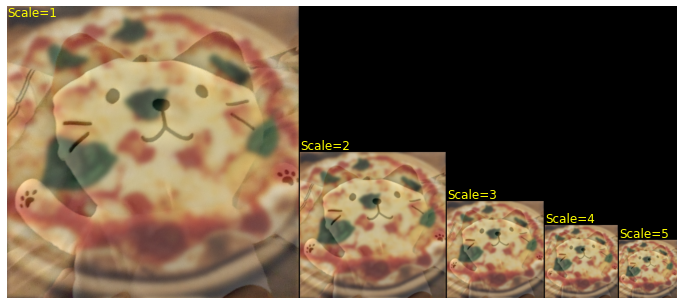
\includegraphics[scale=0.7]{kadai4_3_19.png}
              \end{center}
              \caption{(2)のハイブリッド画像}
          \end{figure}

          \clearpage
          \begin{figure}[h]
              \begin{center}
                  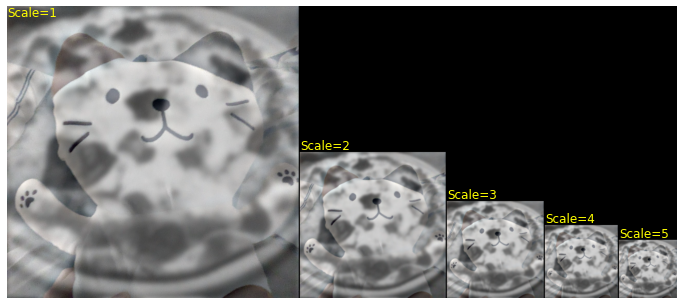
\includegraphics[scale=0.7]{kadai4_3_20.png}
              \end{center}
              \caption{(2)の片方グレースケールのハイブリッド画像}
          \end{figure}

    \item [(3)]画像1と画像4を用いてハイブリッド画像を作成した。
          \begin{figure}[h]
              \begin{center}
                  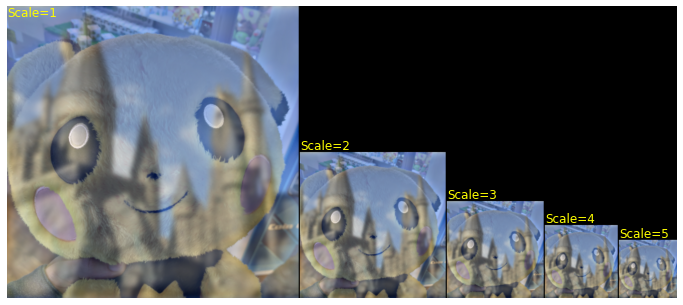
\includegraphics[scale=0.7]{kadai4_3_21.png}
              \end{center}
              \caption{(3)のハイブリッド画像}
          \end{figure}

          \clearpage
          \begin{figure}[h]
              \begin{center}
                  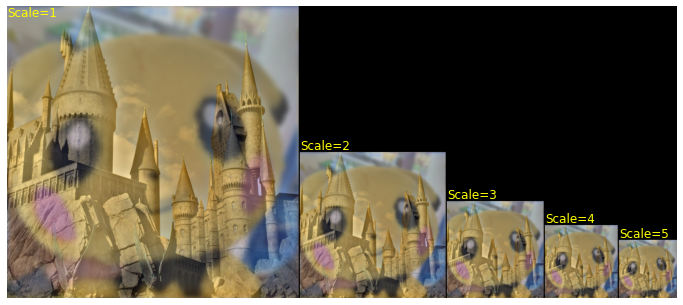
\includegraphics[scale=0.7]{kadai4_3_22.png}
              \end{center}
              \caption{(3)の入れ替えたハイブリッド画像}
          \end{figure}

    \item [(4)]画像2と画像4を用いてハイブリッド画像を作成した。
          \begin{figure}[h]
              \begin{center}
                  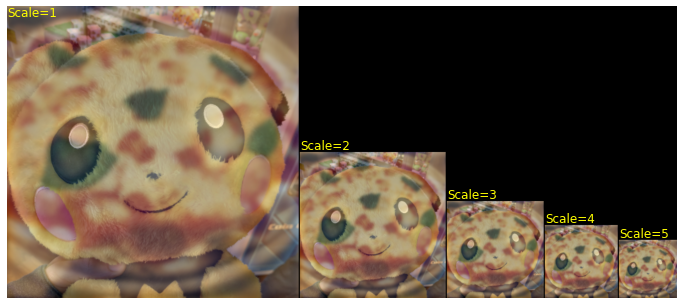
\includegraphics[scale=0.7]{kadai4_3_23.png}
              \end{center}
              \caption{(4)のハイブリッド画像}
          \end{figure}

          \clearpage
          \begin{figure}[h]
              \begin{center}
                  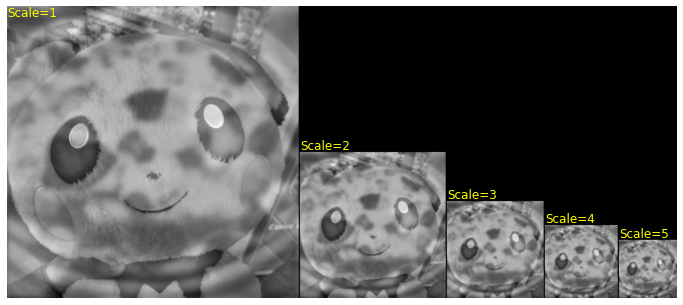
\includegraphics[scale=0.7]{kadai4_3_24.png}
              \end{center}
              \caption{(4)のグレースケールのハイブリッド画像}
          \end{figure}

\end{itemize}
\subsection{検討・考察}

\subsubsection{}
上記の実験の結果より、
画像が大きいとハイパスフィルタの画像がよく見え、画像が小さいとローパスフィルタの画像がよく見えた。

ローパスフィルタとハイパスフィルタのカットオフ周波数の間隔はある程度存在するべきであると考える。
具体的には、今回用いた画像ではローパスフィルタとハイパスフィルタのカットオフ周波数の間隔を0にすると、
どのScaleも両方が同じくらい見える程度だった。

\subsubsection{}
\begin{itemize}
    \item [(1)]図17と図18を比べると、ローパスフィルタの方の画像は明るい色が多く使われている方が、
          認識しやすいことが分かる。今回でいうと、図18の方が認識しやすいと考える。
    \item [(2)]図19と図20を比べると、画像3自体が暗い画像なので、
          もう一つの方の画像をグレースケールにすることにより、認識しやすいハイブリッド画像となっている。
          今回は、図20の方が認識しやすいと考える。
    \item [(3)]図21と図22を比べると、青色と黄色の相性が悪く、黄色の主張が激しいので
          どのScaleも黄色が強くあらわれてしまい、認識しにくくなった。今回は、図21の方が認識しやすいと考える。
    \item [(4)]図23と図24を比べると、元画像が両方黄色が多く含まれていたので、
          グレースケールにしてもしなくても同じ程度の認識のしやすさとなった。
\end{itemize}

\clearpage
\section{まとめ}
本実験では、
画像の2次元フーリエ変換と周波数フィルタリングを実装し、
入力画像やそのパラメータを変化させながら変換結果を評価することで、
フーリエ変換と周波数領域での画像処理について理解することができた。


\clearpage
\appendix
\section{付録}

\begin{lstlisting}[style = py,caption=kadai1]
    #4619055
    from expr3fft import *
    import matplotlib.pyplot as plt
    import copy
    %matplotlib inline
    
    def hybrid_image(im1, im2, cutoff1 = 16, cutoff2 = 16, visu = False):
        """ ハイブリッド画像の作成 
             cutoff1 -- ガウス型ローパスフィルタのカットオフ周波数(cycles/image)
             cutoff2 -- ガウス型ハイパスフィルタのカットオフ周波数(cycles/image)
        """
        # 低周波数領域,高周波領域のカットオフ周波数cutoff1, cutoff2から周波数フィルタ関数を作成
        def lowpass_gauss(u, v, sigma):
            """ ガウス分布型ローパスフィルタ """
            return np.exp(-1.0*(u**2 + v**2)/(2*sigma**2))
    
        def lowpass(u, v): 
            return lowpass_gauss(u, v, 1.2 * cutoff1 / im1.shape[0])
    
        def highpass(u, v): 
            return 1.0 - lowpass_gauss(u, v, 0.63 * cutoff2 / im1.shape[0])
        
        # (1) フーリエ変換
        fshift1 = do_fft(im1)
        fshift2 = do_fft(im2)
        
        # (2) 周波数フィルタリング
        fshift1 = do_ffilter(fshift1, lowpass)
        fshift2 = do_ffilter(fshift2, highpass)
        
        # (3) ハイブリッドイメージの合成
        hybrid_image = do_ifft(fshift1 + fshift2) 
        hybrid_image = array_normalize(hybrid_image)  # 画素値を0~1に正規化
        
        return hybrid_image
    
    W = 512   # 画像サイズ(縦横の画素数)
    im1 = imread("kadai/USJ.jpg")
    im2 = imread("kadai/pizza.jpg")
    im3 = imread("kadai/catcat.jpg")
    im4 = imread("kadai/pichu.jpg")
    
    # 画像のサイズを同じに揃える
    im1 = resize(im1, (W, W))
    im2 = resize(im2, (W, W))
    im3 = resize(im3, (W, W))
    im4 = resize(im4, (W, W))
    
    im5 = copy.copy(im2)
    im6 = copy.copy(im4)
    
    for x in range(0,512):
        for y in range(0,512):
            im5[y,x] = np.dot(im5[y,x],[0.299, 0.587, 0.114])
            im6[y,x] = np.dot(im6[y,x],[0.299, 0.587, 0.114])
    
    #(1)
    for i in range(4):
        for j in range(3):
            plt.figure(figsize=(12, 12))
            him = hybrid_image(im1, im2, cutoff1=4*2**i, cutoff2=8*2**j, visu=False)
            show_hybrid_image(him)
            
    #(2)
    #(2.1)
    plt.figure(figsize=(12, 12))
    him = hybrid_image(im3, im4, cutoff1=16, cutoff2=8, visu=False)
    show_hybrid_image(him)
    
    plt.figure(figsize=(12, 12))
    him = hybrid_image(im4, im3, cutoff1=16, cutoff2=8, visu=False)
    show_hybrid_image(him)
    
    #(2.2)
    plt.figure(figsize=(12, 12))
    him = hybrid_image(im2, im3, cutoff1=16, cutoff2=8, visu=False)
    show_hybrid_image(him)
    
    plt.figure(figsize=(12, 12))
    him = hybrid_image(im5, im3, cutoff1=16, cutoff2=8, visu=False)
    show_hybrid_image(him)
    
    #(2.3)
    plt.figure(figsize=(12, 12))
    him = hybrid_image(im1, im4, cutoff1=16, cutoff2=8, visu=False)
    show_hybrid_image(him)
    
    plt.figure(figsize=(12, 12))
    him = hybrid_image(im4, im1, cutoff1=16, cutoff2=8, visu=False)
    show_hybrid_image(him)
    
    #(2.4)
    plt.figure(figsize=(12, 12))
    him = hybrid_image(im2, im4, cutoff1=16, cutoff2=8, visu=False)
    show_hybrid_image(him)
    
    plt.figure(figsize=(12, 12))
    him = hybrid_image(im5, im6, cutoff1=16, cutoff2=8, visu=False)
    show_hybrid_image(him)
    
\end{lstlisting}


%%%%%%%%%%%%%%%%%%%%%%%%%%%%%%%%%%%%%%%%%%%%%%%%%%%%%%%
\end{document}